\chapter{Uma avaliação do OpenFlow}

Esse capítulo avalia o protocolo OpenFlow através de um sistema de
balanceamento de carga.
Através dos recursos fornecidos pelo protocolo é possível maximizar a justiça
no balanceamento de carga em um serviço HTTP.
Detalhes sobre a implementação e os resultados desse experimentos são 
apresentados nesse capítulo.

\section{Proposta}

Sistemas de balanceamento de carga são baseados em políticas de balanceamento.
Essas políticas podem se aproveitar positivamente da separação do plano de 
dados e do plano de controle e sua flexibilidade.
O presente trabalho apresenta um sistema de balanceamento de carga inteligente
baseado em Redes Definidas por \emph{Software} (SDN).
As políticas de balanceamento são baseadas no trafego da rede, na carga dos 
servidores e no estado corrente do serviço.
Os experimentos mostram que a abordagem em SDN permite um balancemanto de carga
que reduz a carga dos servidores, aumenta a disponibilidade do serviço e 
otimiza a instalação de fluxos no plano de dados.

\section{Introdução}

Os serviços modernos devem ser escaláveis para atender a milhões ou milhares
de clientes.
Para realizar essa tarefa, os serviços devem ser distribuídos em vários
servidores. 
Como consequência, para garantir a experiência do usuário/cliente, o volume
de consultas em processamento por cada servidor deve ser compatível com 
sua capacidade.

Balancemento de carga é um requisito para sistemas distribuídos que se 
escalam através de vários servidores.
Conforme apresentado em \citep{hardeep2010openflow}, balanceamento de carga
em Redes de computadores consiste em uma técnica usada para distribuir a 
carga de trabalho entre vários enlaces ou computadores.
Um balanceamento de carga deve ser transparente para o usuário final e 
permitir que a aplicação seja escalável e flexível.

As soluções atuais são muito caras. 
Normalmente, dispositivos intermediários (\emph{middleboxes}) são utilizados,
no entanto não são customizáveis \citep{richard2011openflow}.
Balanceadores de carga são caros e, em muitos casos, tornam-se um ponto de 
congestionamento da rede \citep{nikhil2010asterix}.
Os dispositivos intermediários para balanceamento de carga não levam em conta
a largura de banda ou a latência da rede.
Contudo, alguns balanceadores não conseguem agrupar as requisições por 
similaridade \citep{richard2011openflow}, nem avaliar diretamente a topologia
da rede como em \citep{nikhil2009plugnserve}.


Uma solução viável seria executar a tarefa de balanceamento de carga em 
comutadores comerciais.
O protocolo OpenFlow permite que, políticas de balanceamento de carga, sejam
aplicadas a rede com baixo custo e que podem se adaptar à aplicação ou serviço.

A solução proposta nessa avaliação, é aproveitar da flexibilidade do plano de
controle separado do plano de dados.
Como uma entidade logicamente centralizada, o controlador possui uma visão 
topológica global da rede \citep{nick2008openflow}.
Os experimentos mostram que a abordagem em SDN a perda de pacotes do serviço
e seu atraso.
A disponibilidade e a vazão da aplicação é maximizada.
As políticas de balanceamento de carga propostos não distribuem igualmente as 
requisições entre os servidores. 
Ao invés disso, elas garantem que a carga de trabalho ao longo dos servidores
da aplicação sejam mais justos e homogênea.

Um sistema de balanceamento de carga corporativo utilizando OpenFlow é 
apresentado em \citep{nikhil2009plugnserve}.
Uma generalização do fluxo de pacotes através de \emph{wildcards} (fluxos
curinga) foi feita em \citep{richard2011openflow}.
Uma medição da latência e da largura de banda é descrita em 
\citep{hardeep2010openflow}.
Um modelo de protocolo para balanceamento de carga foi proposto por 
\citep{charalampos2013modelling}.
Esse trabalho apresenta uma proposta que verifica a carga de servidores de 
aplicação, a fila de requisições (HTTP), a carga prevista e o número de 
requisições respondidads.
Esses parâmetros são a basa do balanceamento de carga. 
Os fluxos de ida e de volta (fluxo reverso) são instalados nos comutadores a
fim de reduzir o número de pacotes enviados ao controlador.

Primeiramente apresentamos o projeto do sistema de balanceamento de carga.
Em seguida, são discutidas as políticas de balanceamento de carga.
Os experimentos e a avaliação dos resultados são apresentados.
Ao final, são discutidos trabalhos futuros e uma conclusão.

\section{Trabalhos relacionados}

Balancemento de carga é importante para serviços que exigem robustês ao dividir
a carga de entrega de pacotes de modo agregado.
O OpenFlow permite criar soluções de baixo custo.
Considerar o balanceamento de carga uma primitiva em Redes de computadores é 
apresentado em \cite{nikhil2010asterix}.

Medições de latência e largura de banda foram feitos através do controlador
NOX em \cite{hardeep2010openflow}.
Abordagens utilizando regras genéricas (\emph{wildcards}) para evitar instalar
separadamente fluxos é apresentado em \cite{richard2011openflow}. 
Esses fluxos reduzem o volume de pacotes enviados para o controlador.

Um balanceamento de carga dinâmico para \emph{cluster} de computadores em 
ambientes virtualizados utilizando OpenFlow é mostrado em 
\citep{chen2014design}.
Um algoritmo de balanceamento de carga chamado \emph{Server-based} (SBLB) 
é proposto. 
Dinamicamente ele recupera dados da carga nos servidores para a tomada de 
decisão do balanceamento de carga. 

A proposta do presente trabalho é uma extensão do módulo de balanceamento
de carga do controlador POX \citep{pox2015}.
São reduzidos a perda de pacotes e o atraso na resposta através da instalação
de fluxos reversos. 
São aumentados a disponibilidade e a largura de banda da rede.
Além disso, a distribuição de carga foi aplicada de maneira mais justa entre
os servidores de aplicação.


\section{Projeto de implementação}

A solução resume-se em um balanceador de carga TCP.
A implementação não lida com DNS (\emph{domain name service}).
O balanceador de carga toma decisões avaliando a carga dos servidores
(\emph{load avarage}), o número de pendências na fila de requisições do 
servidor HTTP e o número requisições já respondidas.
Os dados monitorados pelas políticas de balanceamento de carga foram coletados
através de um comutador \emph{OpenFlow} e através do sistema de arquivos 
distribuído NFS (\emph{Network File Syste}).

O controlador POX \citep{pox2015} foi adotado como base da solução proposta.
A arquitetura baseada em eventos permite que módulos atuem como produtores
e consumidores de eventos.
O módulo \emph{core} encapsula o controle de eventos.
Novos eventos podem ser registrados por outros módulos.

\subsection{Balanceador de carga}

O módulo \emph{load\_balancer} foi implementado como uma classe.
Esse módulo se registra no \emph{core} no momento em que o controlador é 
executado.
Para inicialiar o módulo é necessário informar uma lista de endereços IPs
que representam a lista de servidores a serem balanceados.
Um IP lógico deve ser informado ao módulo ao qual todas as requisições durante
os experimentos serão direcionadas.
Cada requisição direcionada ao IP lógico é direcionada a um dos servidores 
cuja carga, no momento, seja a menor.

\subsection{Fluxo de trabalho do controlador}

Novos pacotes na rede geram pacotes de entrada \emph{PacketIn} no controlador.
O balancedor de carga avalia o novo fluxo e instala uma regra no 
comutador baseado em uma política de balanceamento de carga.
Os demais pacotes similares a esse fluxo são encaminhados para o mesmo 
servidor.
Após algum tempo, os fluxos expiram no comutador, permitindo maior 
dinamismo na rede.

A decisão de qual servidor escolher para encaminhar os pacotes depende 
diretamente da política de balancemanto de carga. 
Através do sistema de arquivos remoto a carga dos servidores foi monitorada.
A tabela \ref{tab:monitor} apresenta os valores coletados de cada servidor.

\begin{table}
\begin{center}
\begin{tabular}{ |c|c|c| } 
 \hline
 Carga média & Fila de pendências & Número de \\ 
  de CPU & do servidor HTTP & requisições respondidas \\
 \hline
\end{tabular}
\end{center}
\label{tab:monitor}
\caption{Dados monitorados de cada servidor HTTP}
\end{table}


O fluxo da execução das requisições feitas ao serviço é mostrado na figura
\ref{fig:balancer-workflow}

\begin{figure}[htb!]
    \centering
    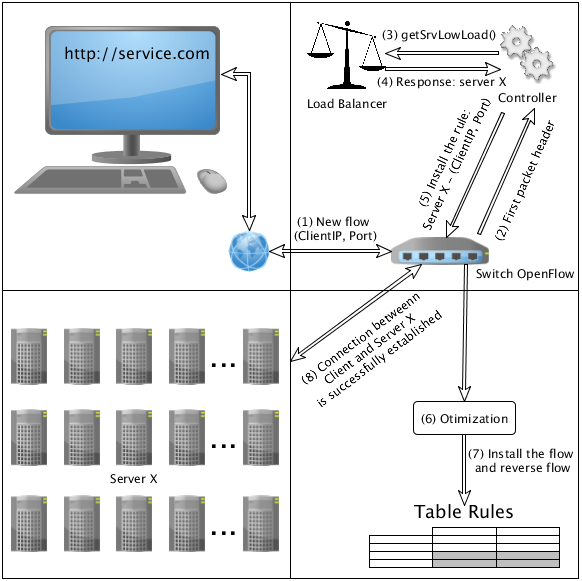
\includegraphics[width=\linewidth]{img/balancer-workflow}
    \caption{Fluxo de execução das requisições ao serviço de balanceamento 
    de carga}
    \label{fig:balancer-workflow}
\end{figure}

\textcolor{red}{Trocar essa imagem dos workflow de balanceamento de carga. 
Fazer no formato de diagrama de sequência.}

\subsection{}

Cinco políticas de balanceamento de carga foram utilizadas pelo módulo para 
distribuir a carga de trabalho entre os servidores.

\begin{enumerate}
    \item Round-robin
    \item Aleatória
    \item Carga
    \item Fila 
    \item Mistura
\end{enumerate}

\emph{Round Robin} é uma política que divide de maneira idêntica o volume de
requisições entre os servidores.

A política de balanceamento Aleatória escolhe a cada nova requisição, 
aleatoriamente, o servidor a responder pela requisição.

A política de balanceamento Carga é baseada em avaliar a carga de CPU 
de cada servidor e encaminhar a requisição para o servidor com a menor 
carga do momento.
    
Fila é uma política de balanceamento que avalia a quantidade de requisições
pendentes na fila de requisições do servidor HTTP.
    
A política de balanceamento Mistura combina as políticas Carga e Fila 
e escolhe o servidor com a menor valor da combinação.

\subsection{Servidor HTTP}

O servidor responsável por responder as requisições HTTP foi o 
\emph{Tornado} \citep{tornado}.
O \emph{Tornado} é um arcabouço e uma biblioteca HTTP assíncrona.
Nos experimentos, o \emph{Tornado} escreve, periodicamente, em um arquivo 
no sistema de arquivos os dados da sua fila de requisições pendentes,
a carga do servidor e o número de requsições já respondidas.
O balanceador de carga lê remotamente esses dados para compor os 
dados avaliados pelas políticas de balancemento de carga.
